\documentclass{article}
\usepackage{tikz}
%Title
\title{Bipartito o Ciclo}
\author{Daniel Bustos}
\begin{document}
\maketitle

Sea $G = (V,E)$ con $|V| = n$. Queremos probar que: $\forall v \in V$, $G-v$ es bipartito $\leftrightarrow$ $G$ es bipartito o ciclo impar.

Probemos la ida:

\textbf{$\forall v \in V$, $G-v$ es bipartito $\rightarrow$ $G$ es bipartito o ciclo impar.}\\

Probémoslo por el contrarrecíproco.\\
\textbf{$G$  no es bipartito ni es ciclo impar $\rightarrow \exists v \in V: G-v $ no es bipartito}
Supongamos que $G$ no es bipartito ni ciclo impar. Esto nos deja dos casos:
\begin{itemize}


\item Si es ciclo par, podemos tomar los vértices impares, y los impares por separado. Dentro de cada uno de estos no hay relaciones, por lo tanto, $G$ es bipartito, lo cual es absurdo porque dijimos que $G$ no lo era. Luego, este caso no puede ocurrir. Por ejemplo:

\begin{center}
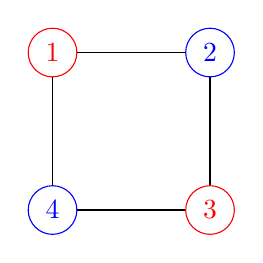
\begin{tikzpicture}
  \node[circle,draw,red] (1) at (0,0) {1};
  \node[circle,draw,blue] (2) at (2,0) {2};
  \node[circle,draw,red] (3) at (2,-2) {3};
  \node[circle,draw,blue] (4) at (0,-2) {4};
  
  \draw (1) -- (2);
  \draw (2) -- (3);
  \draw (3) -- (4);
  \draw (4) -- (1);
\end{tikzpicture}
\end{center}

Se observa que podemos tomar las biparticiones $\{1,3\}$ y $\{2,4\}$ respectivamente.

\item $G$ no es ciclo: En este caso debemos usar algo un poco mas potente. Sabemos por teorema que : Si un grafo G no es bipartito  \leftrightarrow \exists un ciclo impar en G
A partir de esto podemos tomar otros dos subscuentes casos
\item[red] Ciclo impar con cosas sueltas afuera:
begin{center}
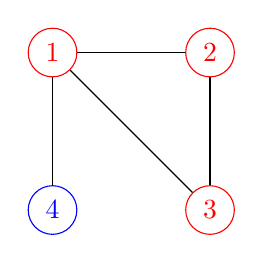
\begin{tikzpicture}
  \node[circle,draw,red] (1) at (0,0) {1};
  \node[circle,draw,red] (2) at (2,0) {2};
  \node[circle,draw,red] (3) at (2,-2) {3};
  \node[circle,draw,blue] (4) at (0,-2) {4};
  
  \draw (1) -- (2);
  \draw (2) -- (3);
  \draw (3) -- (1);
  \draw (4) -- (1);
\end{tikzpicture}
\end{center}
En este caso podemos tomar remover algun vértices de afuera
		
\item[red] Ciclo impar sin nada afuera, pero aristas internas extras


\end{itemize}
Probemos la vuelta: 
\begin{itemize}

	\item Si G es bipartito

\end{itemize}

\textbf{$G$ es bipartito o ciclo impar. $\rightarrow \forall v \in V$, $G-v$ es bipartito} 




\end{document}
